\documentclass{beamer}
\usetheme{Antibes}
\usepackage{xcolor, colortbl}
\usepackage{algorithm}
\usepackage{algpseudocode}
\usepackage{textcomp}
\usepackage{listings}
\usepackage{hyperref}
\usepackage{alltt}
\usepackage{tikz}
\usepackage{framed}
\usepackage{marvosym}
\usepackage{wasysym}
\usepackage{marvosym}
\usepackage{crayola}
\usepackage{mathpartir}
\usepackage{tabularx}
\usepackage[belowskip=-15pt,aboveskip=0pt]{caption}
\usepackage[skins]{tcolorbox}
\usepackage{multicol}
\usetikzlibrary{positioning,shapes,arrows, backgrounds, fit, shadows, automata}
\usetikzlibrary{decorations.markings, calc}
%\usepackage{wasysym}
%\usepackage{marvosym}
\setbeamertemplate{footline}[frame number]
%\usecolortheme{fly}
\usefonttheme{serif}

\title[Sujit]{Lexical Analysis \\
Programming Languages}
\author{Sujit Kumar Chakrabarti}
\institute{IIITB}
\date{}


\definecolor{lightblue}{rgb}{0.8,0.93,1.0} % color values Red, Green, Blue
\definecolor{darkblue}{rgb}{0.4,0.3,1.0} % color values Red, Green, Blue
\definecolor{Blue}{rgb}{0,0,1.0} % color values Red, Green, Blue
\definecolor{darkgreen}{rgb}{0,0.7,0.2} % color values Red, Green, Blue
\definecolor{Red}{rgb}{1,0,0} % color values Red, Green, Blue
\definecolor{Pink}{rgb}{0.7,0,0.2}
\definecolor{links}{HTML}{2A1B81}
\definecolor{mydarkgreen}{HTML}{126215}
\newcommand{\highlight}[1]{{\color{Red}(#1)}}

\newcommand{\myheader}[1]{
	{\color{darkblue}
		\begin{Large}
			\begin{center}
				{#1}
			\end{center}
		\end{Large}
	}
}
\newcommand{\myminorheader}[1]{
	{\color{BrickRed}
		\begin{Large}
			{\fontfamily{\sfdefault}\selectfont\textbf{#1}}
		\end{Large}
	}
}

%\tikzstyle{input} = [coordinate]
%\tikzstyle{output} = [coordinate]


\tikzstyle{bb}=[%
      rectangle, draw=black, thick, fill=OliveGreen!30, drop shadow, align=center,
      text ragged, minimum height=2em, minimum width=2em, inner sep=6pt
]

\tikzstyle{inv}=[%
      rectangle, draw=none,  align=center,
      text ragged, minimum height=2em, minimum width=2em, align=center, inner sep=6pt
]

\tikzstyle{db}=[%
      ellipse, draw=black, thick, fill=pink, drop shadow, align=center,
      text ragged, minimum height=2em, inner sep=6pt
]

\tikzstyle{jn}=[%
      inner sep=0cm, outer sep=0cm
]

\tikzstyle{io}=[%
      trapezium, trapezium left angle=60, trapezium right angle=120, draw=black, thick, fill=brown, drop shadow,
      text ragged, minimum height=2em, minimum width=2em, inner sep=6pt, align=center
]

\tikzstyle{glio}=[%
      trapezium, trapezium left angle=60, trapezium right angle=120, draw=red, line width = 1mm, fill=brown, drop shadow,
      text ragged, minimum height=2em, minimum width=2em, inner sep=6pt
]
\tikzstyle{gl}=[%
      rectangle, draw=red, line width = 1mm, fill=lightblue, drop shadow,
      text ragged, minimum height=2em, minimum width=2em, inner sep=6pt
]

\tikzstyle{en}=[%
      rectangle, draw=black, thick, fill=none,
      text ragged, minimum height=2em, minimum width=2em, inner sep=6pt
]

\tikzstyle{sh}=[%
      rectangle, draw=gray, thick, fill=none, color = gray,
      text ragged, minimum height=2em, minimum width=2em, inner sep=6pt
]


\lstdefinestyle{javacode}{
	language = Java,
	basicstyle = \ttfamily\scriptsize,
	stringstyle = \ttfamily,
	keywordstyle=\color{Blue}\bfseries,
	identifierstyle=\color{Pink},
	commentstyle=\color{darkgreen},
	frame=single,
	frameround=tttt,
%	numbers=left
	showstringspaces=false
}

\lstdefinestyle{camlcode}{
	language = Caml,
	basicstyle = \scriptsize\ttfamily,
	stringstyle = \color{red}\ttfamily,
	keywordstyle=\color{Blue}\bfseries,
	identifierstyle=\ttfamily,
	frame=single,
	frameround=tttt,
	numbers=none,
	showstringspaces=false,
	escapeinside={(*@}{@*)}
}

\lstdefinestyle{outputcode}{
	language = bash,
	backgroundcolor = \color{black},
	basicstyle = \tiny\ttfamily\color{white},
	stringstyle = \color{red}\ttfamily,
	keywordstyle=\color{white}\bfseries,
	identifierstyle=\ttfamily,
	frameround=tttt,
	numbers=none,
	showstringspaces=false,
	escapeinside={(*@}{@*)}
}

\newtcolorbox{myframe}[2][]{%
  enhanced,colback=white,colframe=black,coltitle=black,
  sharp corners,boxrule=0.4pt,
  fonttitle=\itshape,
  attach boxed title to top left={yshift=-0.3\baselineskip-0.4pt,xshift=2mm},
  boxed title style={tile,size=minimal,left=0.5mm,right=0.5mm,
    colback=white,before upper=\strut},
  title=#2,#1
}

\begin{document}
\maketitle


% frame begin %%%%%%%%%%%%%%%%%%%%%%%%
\begin{frame}{Finite State Automata (FSA)}
\begin{enumerate}
	\item Non-deterministic FSA
	\item Deterministic FSA
\end{enumerate}
\end{frame}
% frame end %%%%%%%%%%%%%%%%%%%%%%%%

% frame begin %%%%%%%%%%%%%%%%%%%%%%%%
\begin{frame}{Non-Deterministic FSA (NFA)}

\myminorheader{Example 1}
\begin{center}
\resizebox{!}{0.2\textheight}{%
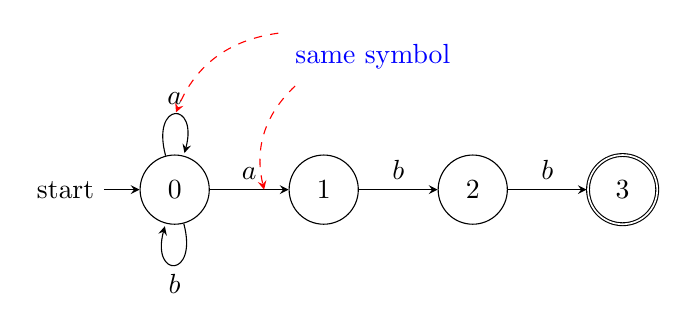
\begin{tikzpicture}[auto,
    ->,
    >=stealth
  ]
    \node[initial, state]   (0)                {$0$};
    \node[state]            (1) [right = of 0] {$1$};
    \node[state] (2) [right = of 1] {$2$};
    \node[state, accepting] (3) [right = of 2] {$3$};
    
    \path (0) edge[loop above] node {$a$} (0)
          (0) edge[loop below] node {$b$} (0)
          (0) edge node {$a$} (1)
          (1) edge node {$b$} (2)
          (2) edge node {$b$} (3)
    ;

\pause
	\node[jn, above=0.5cm of 0] (j1) {};
	\node[inv, above right=of 0] (l1) {\color{Blue}same symbol};
	
	\draw[->, Red, dashed, bend right] (l1) to (j1);
	
	\coordinate(e1) at ($(0)!0.6!(1)$);
	\draw[->, Red, dashed, bend right] (l1) to (e1);
  \end{tikzpicture}
}

\end{center}
\pause
\textbf{Language:} \pause$(a|b)\star abb$


\end{frame}
% frame end %%%%%%%%%%%%%%%%%%%%%%%%


% frame begin %%%%%%%%%%%%%%%%%%%%%%%%
\begin{frame}{Non-Deterministic FSA (NFA)}
\myminorheader{Example 2}
\begin{center}
\resizebox{0.4\textwidth}{!}{%
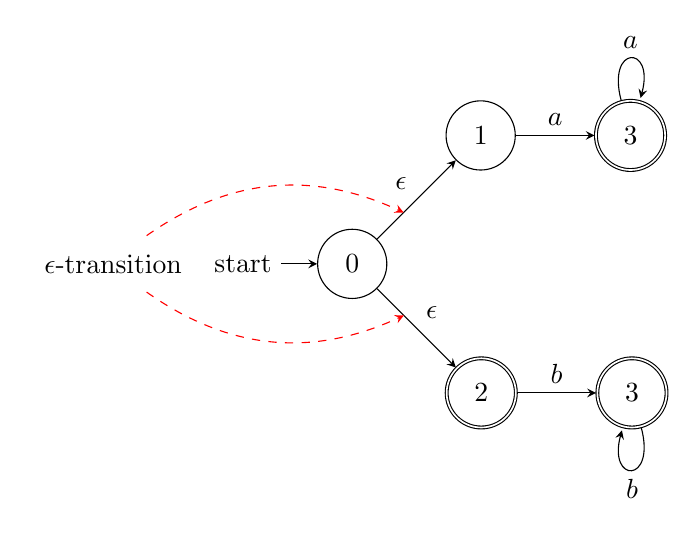
\begin{tikzpicture}[auto,
    ->,
    >=stealth
  ]
    \node[initial, state]   (0)                {$0$};
    \node[state]            (1) [above right = of 0] {$1$};
    \node[state, accepting] (2) [below right = of 0] {$2$};
    \node[state, accepting] (3) [right = of 1] {$3$};
    \node[state, accepting] (4) [right = of 2] {$3$};
    
    \path (0) edge node {$\epsilon$} (1)
          (0) edge node {$\epsilon$} (2)
          (1) edge node {$a$} (3)
          (2) edge node {$b$} (4)
          (3) edge[loop above] node {$a$} (3)
          (4) edge[loop below] node {$b$} (4)
          
    ;
\pause
	\node[inv, left=1.5cm of 0](l1){$\epsilon$-transition};
	\coordinate(e1) at ($(0)!0.4!(1)$);
	\coordinate(e2) at ($(0)!0.4!(2)$);
	\draw[->, Red, dashed, bend left] (l1) to (e1);
	\draw[->, Red, dashed, bend right] (l1) to (e2);
    
  \end{tikzpicture}
}

\end{center}
\textbf{Language:} $aa\star|bb\star$

\end{frame}
% frame end %%%%%%%%%%%%%%%%%%%%%%%%

% frame begin %%%%%%%%%%%%%%%%%%%%%%%%
\begin{frame}{Non-Deterministic FSA (NFA)}
\begin{itemize}
	\item Finite set of states -- ($S$)
	\item Alphabet - ($\sum$)
	\item Transition function ($T : S \times \sum \rightarrow 2^S$)
	\item Initial state ($S_0$)
	\item Final/accepting states ($F \subseteq S$)
	\pause
	\item \textbf{Acceptance of a string: }When there exists a path corresponding to the input leading to an accepting state.
\end{itemize}

\pause
\myminorheader{Specific Properties}
\begin{itemize}
	\item The same state can transition to more than one states on the same symbol
	\item $\epsilon$-transitions
\end{itemize}

\end{frame}
% frame end %%%%%%%%%%%%%%%%%%%%%%%%

% frame begin %%%%%%%%%%%%%%%%%%%%%%%%
\begin{frame}{Deterministic FSA (DFA)}
\begin{itemize}
	\item Finite set of states -- ($S$)
	\item Alphabet - ($\sum$)
	\item Transition function ($T : S \times \sum \rightarrow S$)
	\item Initial state ($S_0$)
	\item Final/accepting states ($F \subseteq S$)
	\item \textbf{Acceptance of a string: }When there exists a path corresponding to the input leading to an accepting state.
\end{itemize}

\pause
\myminorheader{Specific Properties}
\begin{itemize}
	\item Only one next-state on the same symbol
	\item No $\epsilon$-transitions
\end{itemize}

\end{frame}
% frame end %%%%%%%%%%%%%%%%%%%%%%%%

% frame begin %%%%%%%%%%%%%%%%%%%%%%%%
\begin{frame}{Deterministic FSA (DFA)}

\myminorheader{Example 1}

\begin{center}
\resizebox{!}{0.2\textheight}{%
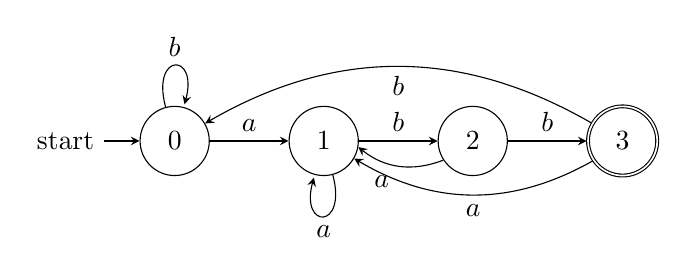
\begin{tikzpicture}[auto,
    ->,
    >=stealth
  ]
    \node[initial, state]   (0)                {$0$};
    \node[state]            (1) [right = of 0] {$1$};
    \node[state] (2) [right = of 1] {$2$};
    \node[state, accepting] (3) [right = of 2] {$3$};
    
    \path (0) edge[loop above] node {$b$} (0)
          (0) edge node {$a$} (1)
          (1) edge[loop below] node {$a$} (1)
          (1) edge node {$b$} (2)
          (2) edge node {$b$} (3)
          (2) edge[bend left] node {$a$} (1.350)
          (3) edge[bend left] node {$a$} (1.330)
          (3) edge[bend right] node {$b$} (0)
    ;
    
  \end{tikzpicture}
}

\end{center}
\pause
\textbf{Language:} \pause$(a|b)\star abb$


\end{frame}
% frame end %%%%%%%%%%%%%%%%%%%%%%%%

% frame begin %%%%%%%%%%%%%%%%%%%%%%%%
\begin{frame}{NFA and DFA}
\begin{itemize}
	\item NFAs: Often more readable
	\item NFAs: Usually have fewer states
	\pause
	\item DFAs: Less readable
	\item DFAs: Larger number of states
	\item DFAs: Faster to simulate
	\pause
	\item Equally expressive $\equiv$ Regular expressions (Regular languages)
\end{itemize}
\end{frame}
% frame end %%%%%%%%%%%%%%%%%%%%%%%%

% frame begin %%%%%%%%%%%%%%%%%%%%%%%%
\begin{frame}{Lexical Analysis Process}
\begin{center}
\resizebox{0.7\textwidth}{!}{%
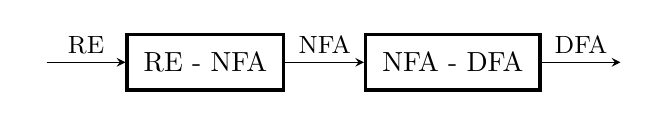
\begin{tikzpicture}[auto,
    ->,
  %  shorten >=2pt,
    >=stealth,
  %  node distance=1cm,
    bb/.style={%
      rectangle, draw=black, very thick, fill=white,
      text ragged, minimum height=2em, inner sep=6pt, align=center
    },
]
    \node      (0)                {};
    \node[bb]  (1) [right = of 0] {RE - NFA};
    \node[bb]  (2) [right = of 1] {NFA - DFA};
    \node      (3) [right = of 2] {};

\begin{small}
    \path (0) edge node[align=center] {RE}  (1)
          (1) edge node[align=center] {NFA} (2)
          (2) edge node[align=center] {DFA} (3)
    ;
\end{small}
  \end{tikzpicture}
}

\end{center}

\end{frame}
% frame end %%%%%%%%%%%%%%%%%%%%%%%%

% frame begin %%%%%%%%%%%%%%%%%%%%%%%%
\begin{frame}{Simulating FSAs}

\myminorheader{Representating \textit{transition function} using transition tables}
\begin{center}
\resizebox{!}{0.2\textheight}{%
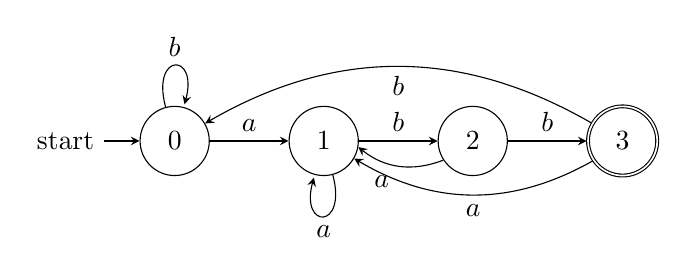
\begin{tikzpicture}[auto,
    ->,
    >=stealth
  ]
    \node[initial, state]   (0)                {$0$};
    \node[state]            (1) [right = of 0] {$1$};
    \node[state] (2) [right = of 1] {$2$};
    \node[state, accepting] (3) [right = of 2] {$3$};
    
    \path (0) edge[loop above] node {$b$} (0)
          (0) edge node {$a$} (1)
          (1) edge[loop below] node {$a$} (1)
          (1) edge node {$b$} (2)
          (2) edge node {$b$} (3)
          (2) edge[bend left] node {$a$} (1.350)
          (3) edge[bend left] node {$a$} (1.330)
          (3) edge[bend right] node {$b$} (0)
    ;
    
  \end{tikzpicture}
}

\end{center}

\textbf{Transition Table:}
\begin{center}
\begin{tabular}{c | c | c }
\hline
\textbf{State} & \textbf{a}        & \textbf{b}     \\
\hline
\onslide<1->0              & \onslide<2->1          & \onslide<2-> 0\\
\onslide<1->1              & \onslide<2->1              & \onslide<2-> 2\\
\onslide<1->2              & \onslide<2->1              & \onslide<2-> 3\\
\onslide<1->3              & \onslide<2->1              & \onslide<2-> 0
\end{tabular}
\end{center}
\end{frame}
% frame end %%%%%%%%%%%%%%%%%%%%%%%%


% frame begin %%%%%%%%%%%%%%%%%%%%%%%%
\begin{frame}{Simulating FSAs}

\myminorheader{Representating \textit{transition function} using transition tables}
\begin{center}
\resizebox{!}{0.2\textheight}{%
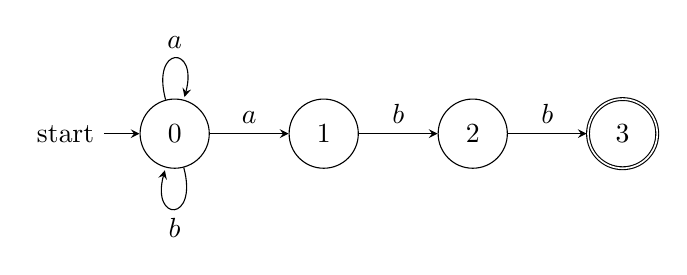
\begin{tikzpicture}[auto,
    ->,
    >=stealth
  ]
    \node[initial, state]   (0)                {$0$};
    \node[state]            (1) [right = of 0] {$1$};
    \node[state] (2) [right = of 1] {$2$};
    \node[state, accepting] (3) [right = of 2] {$3$};
    
    \path (0) edge[loop above] node {$a$} (0)
          (0) edge[loop below] node {$b$} (0)
          (0) edge node {$a$} (1)
          (1) edge node {$b$} (2)
          (2) edge node {$b$} (3)
    ;
    
  \end{tikzpicture}
}

\end{center}

\textbf{Transition Table:}
\begin{center}
\begin{tabular}{c | c | c }
\hline
\textbf{State} & \textbf{a}        & \textbf{b}     \\
\hline
\onslide<1->0              & \onslide<2->\{0, 1\}          & \onslide<2->\{0\} \\
\onslide<1->1              & \onslide<2->\{\}              & \onslide<2->\{2\} \\
\onslide<1->2              & \onslide<2->\{\}              & \onslide<2->\{3\} \\
\onslide<1->3              & \onslide<2->\{\}              & \onslide<2->\{\}
\end{tabular}
\end{center}
\end{frame}
% frame end %%%%%%%%%%%%%%%%%%%%%%%%

% frame begin %%%%%%%%%%%%%%%%%%%%%%%%
\begin{frame}{NFA from Regular Expressions}
\myheader{McNaughton-Yamada-Thompson Algorithm}

\myminorheader{Basis}

$\epsilon$ 
\begin{center}
\resizebox{0.6\textwidth}{!}{%
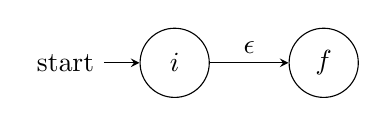
\begin{tikzpicture}[auto,
    ->,
    >=stealth
  ]
    \node[initial, state]   (0)                {$i$};
    \node[state]            (1) [right = of 0] {$f$};
    
    \path (0) edge node {$\epsilon$} (1)
    ;
    
  \end{tikzpicture}
}

\end{center}

$a \in \sum$ 
\begin{center}
\resizebox{0.6\textwidth}{!}{%
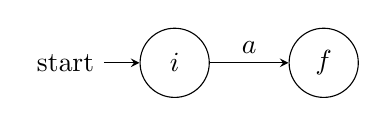
\begin{tikzpicture}[auto,
    ->,
    >=stealth
  ]
    \node[initial, state]   (0)                {$i$};
    \node[state]            (1) [right = of 0] {$f$};
    
    \path (0) edge node {$a$} (1)
    ;
    
  \end{tikzpicture}
}

\end{center}
\end{frame}
% frame end %%%%%%%%%%%%%%%%%%%%%%%%

% frame begin %%%%%%%%%%%%%%%%%%%%%%%%
\begin{frame}{Simulation of DFA}
\footnotesize
\begin{algorithmic}[0]
\Procedure{simDFA}{$D$, $inp$}
\pause
  \State $s \gets D.s_0$
  \While{there is input left}
    \State $c \gets$ \Call{nextChar}{}
    \State $s \gets$ $D$.\Call{move}{$s$, $c$}
    \If{$s$ = \textbf{nil}}
      \State \textbf{break}
    \EndIf
  \EndWhile
  \If{$s \in D.F$}
    \State \textbf{return true}
  \Else
    \State \textbf{return} \textbf{false}
  \EndIf
\EndProcedure

\end{algorithmic}

\end{frame}
% frame end %%%%%%%%%%%%%%%%%%%%%%%%


% frame begin %%%%%%%%%%%%%%%%%%%%%%%%
\begin{frame}{Simulation of NFA}
\begin{algorithmic}[0]
\Procedure{simNFA}{$N$, $inp$}
\pause
  \State $S \gets$ \Call{$\epsilon$-closure}{$N.s_0$}
  \State $c \gets$ \Call{nextChar}{}
  \While{there is input left}
    \State $T' \gets$ \Call{move}{$S$, $c$}
    \State $S \gets$ \Call{$\epsilon$-closure}{$T'$}
    \State $c \gets$ \Call{nextChar}{}
  \EndWhile
  \If{$S \cap N.F \neq \{\}$}
    \State \textbf{return true}
  \Else
    \State \textbf{return} \textbf{false}
  \EndIf
\EndProcedure

\end{algorithmic}

\end{frame}
% frame end %%%%%%%%%%%%%%%%%%%%%%%%

% frame begin %%%%%%%%%%%%%%%%%%%%%%%%
\begin{frame}{Computing $\epsilon$-closure}
\footnotesize
\begin{algorithmic}[0]
\Procedure{$\epsilon$-closure}{$s$}
\pause
  \State $stack \gets$ \Call{copy}{$s$}
  \State $ep \gets$ \Call{copy}{$s$}
  \While{$stack$ is not empty}
    \State $t \gets stack$.\Call{pop}{}
    \State $U \gets \{u : u \in M.Trans[t, \epsilon]\}$
    \For{$u \in U$}
      \If{$u \notin ep$}
        \State $ep$.\Call{add}{$u$}
        \State $stack$.\Call{push}{$u$}
      \EndIf
    \EndFor
  \EndWhile
  \State \textbf{return} $ep$
\EndProcedure

\end{algorithmic}

\end{frame}
% frame end %%%%%%%%%%%%%%%%%%%%%%%%

% frame begin %%%%%%%%%%%%%%%%%%%%%%%%
\begin{frame}{NFA to DFA}
\begin{footnotesize}
\begin{algorithmic}[0]
\Procedure{NFA2DFA}{$N$}
\pause
  \State $s_0' \gets$ \Call{$\epsilon$-closure}{$N.s_0$}
  \State add $s_0'$ to $D.states$
  \State \Call{unmark}{$s_0'$}
  \While{there is unmarked state $T$ in $D.states$}
    \State \Call{mark}{$T$}
    \ForAll{$a \in \sum$}
    	  \State $T' \gets$ \Call{move}{$T$, $a$}
      \State $\mathcal{U} \gets$ \Call{$\epsilon$-closure}{$T'$}
      \If{$\mathcal{U} \notin D.states$}
        \State add $\mathcal{U}$ to $D.states$
        \State \Call{unmark}{$\mathcal{U}$}
      \EndIf
    \EndFor
  \EndWhile
  \State \textbf{return} $D$
\EndProcedure

\end{algorithmic}
\end{footnotesize}
\end{frame}
% frame end %%%%%%%%%%%%%%%%%%%%%%%%

% frame begin %%%%%%%%%%%%%%%%%%%%%%%%
\begin{frame}{NFA to DFA}
\myminorheader{Example}

\textbf{NFA:}

\begin{center}
\resizebox{0.6\textwidth}{!}{%
\begin{tikzpicture}[auto,
    ->,
    >=stealth
  ]
    \node[initial, state]   (0)                       {$0$};
    \node[state]            (1)  [right = of 0]       {$1$};
    \node[state]            (2)  [above right = of 1] {$2$};
    \node[state]            (3)  [right = of 2]       {$3$};
    \node[state]            (4)  [below right = of 1] {$4$};
    \node[state]            (5)  [right = of 4]       {$5$};
    \node[state]            (6)  [below right = of 3] {$6$};
    \node[state]            (7)  [right = of 6]       {$7$};
    \node[state]            (8)  [right = of 7]       {$8$};
    \node[state]            (9)  [right = of 8]       {$9$};
    \node[state, accepting] (10) [right = of 9]       {$10$};
    
    \path (0) edge node {$\epsilon$} (1)
          (0) edge[bend right = 60] node {$\epsilon$} (7)
          (1) edge node {$\epsilon$} (2)
          (1) edge node {$\epsilon$} (4)
          (2) edge node {$a$} (3)
          (4) edge node {$b$} (5)
          (3) edge node {$\epsilon$} (6)
          (5) edge node {$\epsilon$} (6)
          (6) edge node {$\epsilon$} (7)
          (6.90) edge[bend right=90, min distance = 3 cm] node {$\epsilon$} (1.90)
          (7) edge node {$a$} (8)
          (8) edge node {$b$} (9)
          (9) edge node {$b$} (10)
          
          
    ;
    
  \end{tikzpicture}
}
\end{center}

\pause
\textbf{DFA:}
\begin{center}
\resizebox{0.5\textwidth}{!}{%
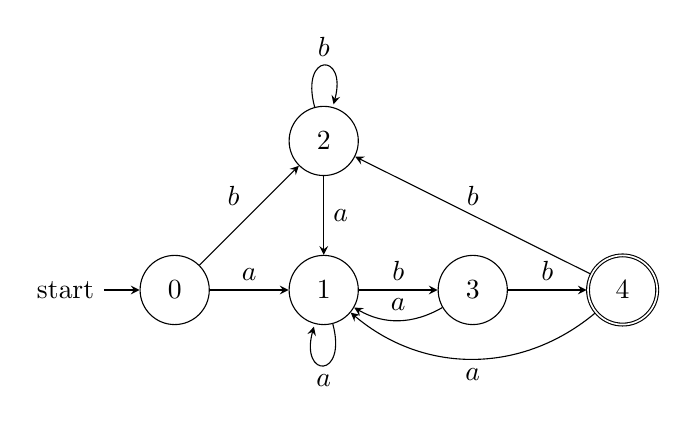
\begin{tikzpicture}[auto,
    ->,
    >=stealth
  ]
    \node[initial, state]   (0)                 {$0$};
    \node[state]            (1)  [right = of 0] {$1$};
    \node[state]            (2)  [above = of 1] {$2$};
    \node[state]            (3)  [right = of 1] {$3$};
    \node[state, accepting] (4)  [right = of 3] {$4$};
    
    \path (0) edge node {$a$} (1)
          (0) edge node {$b$} (2)
          (1) edge node {$b$} (3)
          (1) edge[loop below] node {$a$} (1)
          (2) edge node {$a$} (1)
          (2) edge[loop above] node {$b$} (2)
          (3) edge[bend left] node[above] {$a$} (1)
          (3) edge node {$b$} (4)
          (4) edge[bend left=40] node {$a$} (1)
          (4) edge node[above] {$b$} (2)
    ;
    
  \end{tikzpicture}
}
\end{center}
\end{frame}
% frame end %%%%%%%%%%%%%%%%%%%%%%%%

% frame begin %%%%%%%%%%%%%%%%%%%%%%%%
\begin{frame}{Implementation of Lexical Analysis}
{Manual Implementation of Lexical Analysers -- Example}
\begin{center}
\begin{tabular}{|c|c|c|c|c|c|c|c|}
\hline
\cellcolor{red!75}i & \cellcolor{red!25}n & t & e & g & r & a & l \\
\hline
\end{tabular}
\end{center}

\begin{center}
\resizebox{0.7\textwidth}{!}{%
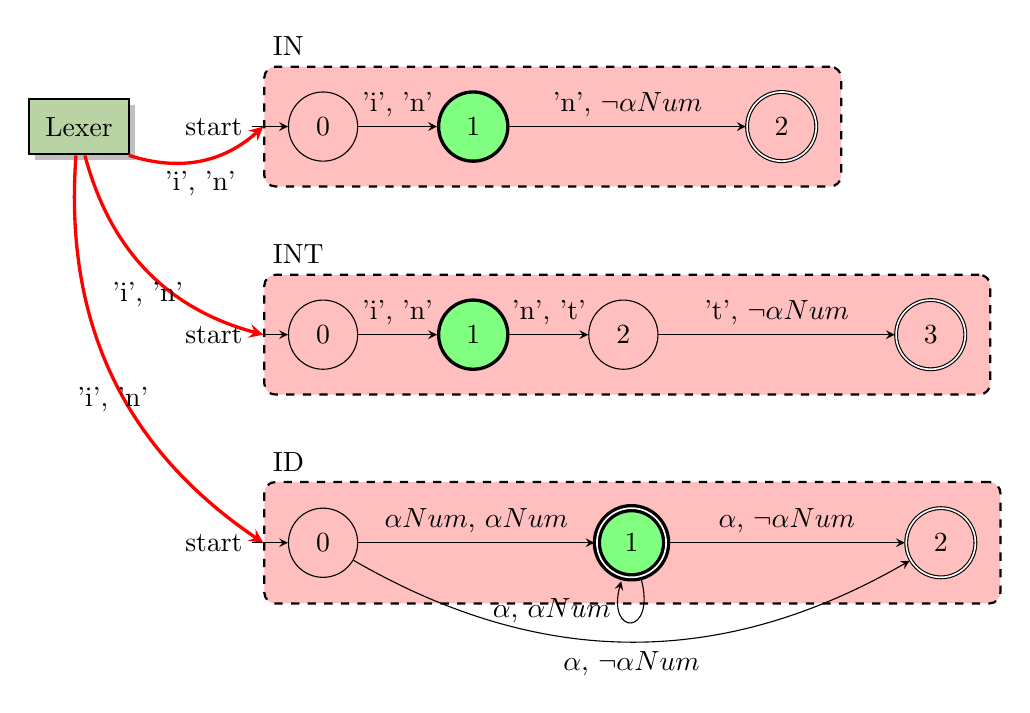
\begin{tikzpicture}[auto,
    ->,
    >=stealth,
    ,
    dead/.style={%
      rectangle, rounded corners=1.5mm, draw=gray, thick, fill=gray!25, drop shadow,align=center,
      text ragged, minimum height=2em, minimum width=2em, inner sep=6pt, outer sep=3pt
    },
    fun/.style = {%
      dashed, draw=black, thick, fill=red!25, rounded corners, rectangle, inner sep=.3cm
    },
    deadfun/.style = {%
      dashed, draw=gray, thick, fill=gray!25, rounded corners, rectangle, inner sep=.3cm
    }
  ]

    \node[bb] (lexer)                           {Lexer};
% IN  
    \node[initial, state]   (10) [right = of lexer, xshift=1cm]          {$0$};
    \node[state, very thick, fill=green!50]            (11) [right = of 10]             {$1$};
    \node[state, accepting] (12) [right = of 11, xshift=2cm] {$2$};
    
    \path (10) edge node {'i', 'n'} (11)
          (11) edge node {'n', $\neg\alpha Num$} (12)
    ;

% INT
    \node[initial, state]   (20) [below = of 10, yshift = -0.75cm] {$0$};
    \node[state, very thick, fill=green!50]            (21) [right = of 20] {$1$};
    \node[state]            (22) [right = of 21] {$2$};
    \node[state, accepting] (23) [right = of 22, xshift=2cm] {$3$};
    
    \path (20) edge node {'i', 'n'} (21)
          (21) edge node {'n', 't'} (22)
          (22) edge node {'t', $\neg\alpha Num$} (23)
    ;
    
%ID
    \node[initial, state]   (30) [below = of 20, yshift = -0.75cm] {$0$};
    \node[state, accepting, very thick, fill=green!50]            (31) [right = of 30, xshift=2cm] {$1$};
    \node[state, accepting]            (32) [right = of 31, xshift=2cm] {$2$};
    
    \path (30) edge node {$\alpha Num$, $\alpha Num$} (31)
          (31) edge[loop below] node[near end, left] {$\alpha$, $\alpha Num$} (31)
          (31) edge node[above] {$\alpha$, $\neg\alpha Num$} (32)
          (30) edge[bend right] node[below] {$\alpha$, $\neg\alpha Num$} (32)
    ;
    
    \begin{pgfonlayer}{background}
      \node[fun] (in)[fit = (10) (11) (12)] {};
      \node[fun] (int)[fit = (20) (21) (22) (23)] {};
      \node[fun] (id)[fit = (30) (31) (32)] {};
      \node[above right] at (in.north west){IN};
      \node[above right] at (int.north west){INT};
      \node[above right] at (id.north west){ID};

    \end{pgfonlayer}
    
	\draw[->, very thick, red, bend right] (lexer) to node[below, black]{'i', 'n'} (in.west);
	\draw[->, very thick, red, bend right] (lexer) to node[below, black]{'i', 'n'} (int.west);
	\draw[->, very thick, red, bend right] (lexer) to node[below, black]{'i', 'n'} (id.west);
	    
  \end{tikzpicture}
}

\end{center}

\end{frame}
% frame end %%%%%%%%%%%%%%%%%%%%%%%%


% frame begin %%%%%%%%%%%%%%%%%%%%%%%%
\begin{frame}{Implementation of Lexical Analysis}
{Manual Implementation of Lexical Analysers -- Example}
\begin{center}
\begin{tabular}{|c|c|c|c|c|c|c|c|}
\hline
i & \cellcolor{red!75}n & \cellcolor{red!25}t & e & g & r & a & l \\
\hline
\end{tabular}
\end{center}

\begin{center}
\resizebox{0.7\textwidth}{!}{%
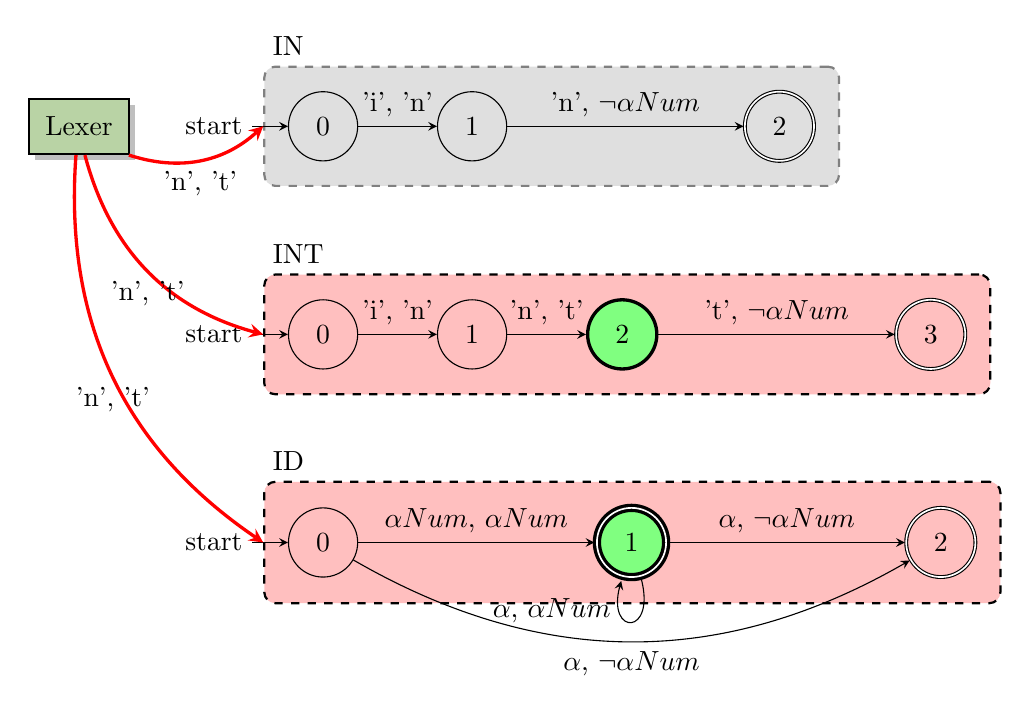
\begin{tikzpicture}[auto,
    ->,
    >=stealth,
    ,
    dead/.style={%
      rectangle, rounded corners=1.5mm, draw=gray, thick, fill=gray!25, drop shadow,align=center,
      text ragged, minimum height=2em, minimum width=2em, inner sep=6pt, outer sep=3pt
    },
    fun/.style = {%
      dashed, draw=black, thick, fill=red!25, rounded corners, rectangle, inner sep=.3cm
    },
    deadfun/.style = {%
      dashed, draw=gray, thick, fill=gray!25, rounded corners, rectangle, inner sep=.3cm
    }
  ]

    \node[bb] (lexer)                           {Lexer};
% IN  
    \node[initial, state]   (10) [right = of lexer, xshift=1cm]          {$0$};
    \node[state]            (11) [right = of 10]             {$1$};
    \node[state, accepting] (12) [right = of 11, xshift=2cm] {$2$};
    
    \path (10) edge node {'i', 'n'} (11)
          (11) edge node {'n', $\neg\alpha Num$} (12)
    ;

% INT
    \node[initial, state]   (20) [below = of 10, yshift = -0.75cm] {$0$};
    \node[state]            (21) [right = of 20] {$1$};
    \node[state, very thick, fill=green!50]            (22) [right = of 21] {$2$};
    \node[state, accepting] (23) [right = of 22, xshift=2cm] {$3$};
    
    \path (20) edge node {'i', 'n'} (21)
          (21) edge node {'n', 't'} (22)
          (22) edge node {'t', $\neg\alpha Num$} (23)
    ;
    
%ID
    \node[initial, state]   (30) [below = of 20, yshift = -0.75cm] {$0$};
    \node[state, accepting, very thick, fill=green!50]            (31) [right = of 30, xshift=2cm] {$1$};
    \node[state, accepting]            (32) [right = of 31, xshift=2cm] {$2$};
    
    \path (30) edge node {$\alpha Num$, $\alpha Num$} (31)
          (31) edge[loop below] node[near end, left] {$\alpha$, $\alpha Num$} (31)
          (31) edge node[above] {$\alpha$, $\neg\alpha Num$} (32)
          (30) edge[bend right] node[below] {$\alpha$, $\neg\alpha Num$} (32)
    ;
    
    \begin{pgfonlayer}{background}
      \node[deadfun] (in)[fit = (10) (11) (12)] {};
      \node[fun] (int)[fit = (20) (21) (22) (23)] {};
      \node[fun] (id)[fit = (30) (31) (32)] {};
      \node[above right] at (in.north west){IN};
      \node[above right] at (int.north west){INT};
      \node[above right] at (id.north west){ID};

    \end{pgfonlayer}
    
	\draw[->, very thick, red, bend right] (lexer) to node[below, black]{'n', 't'} (in.west);
	\draw[->, very thick, red, bend right] (lexer) to node[below, black]{'n', 't'} (int.west);
	\draw[->, very thick, red, bend right] (lexer) to node[below, black]{'n', 't'} (id.west);
	    
  \end{tikzpicture}
}

\end{center}

\end{frame}
% frame end %%%%%%%%%%%%%%%%%%%%%%%%

% frame begin %%%%%%%%%%%%%%%%%%%%%%%%
\begin{frame}{Implementation of Lexical Analysis}
{Manual Implementation of Lexical Analysers -- Example}
\begin{center}
\begin{tabular}{|c|c|c|c|c|c|c|c|}
\hline
i & n & \cellcolor{red!75}t & \cellcolor{red!25}e & g & r & a & l \\
\hline
\end{tabular}
\end{center}

\begin{center}
\resizebox{0.7\textwidth}{!}{%
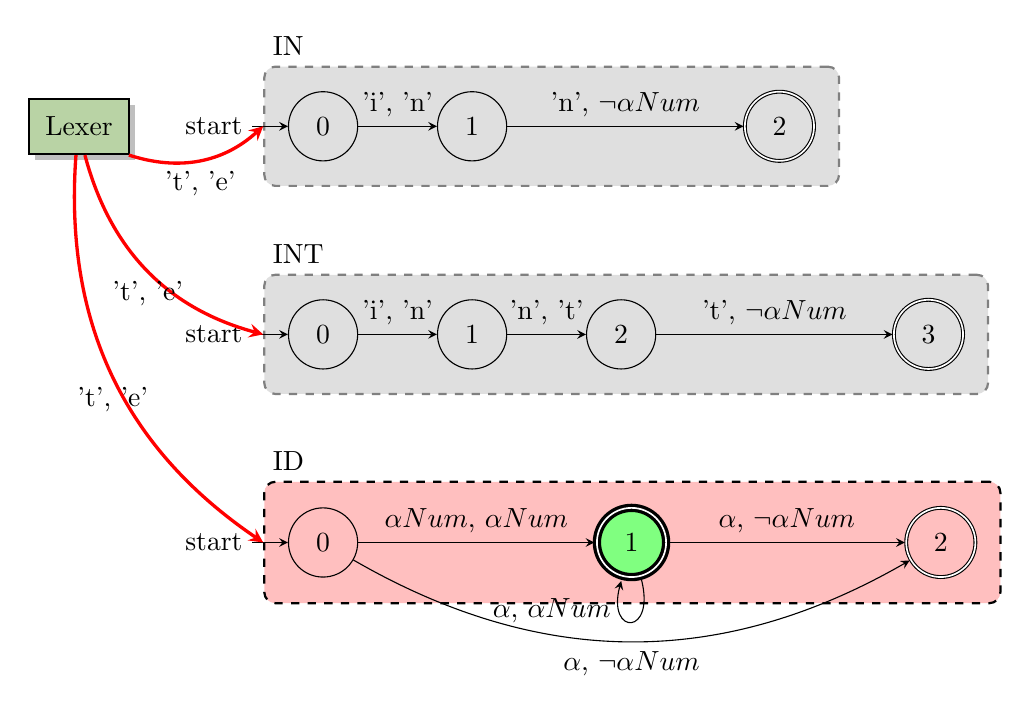
\begin{tikzpicture}[auto,
    ->,
    >=stealth,
    ,
    dead/.style={%
      rectangle, rounded corners=1.5mm, draw=gray, thick, fill=gray!25, drop shadow,align=center,
      text ragged, minimum height=2em, minimum width=2em, inner sep=6pt, outer sep=3pt
    },
    fun/.style = {%
      dashed, draw=black, thick, fill=red!25, rounded corners, rectangle, inner sep=.3cm
    },
    deadfun/.style = {%
      dashed, draw=gray, thick, fill=gray!25, rounded corners, rectangle, inner sep=.3cm
    }
  ]

    \node[bb] (lexer)                           {Lexer};
% IN  
    \node[initial, state]   (10) [right = of lexer, xshift=1cm]          {$0$};
    \node[state]            (11) [right = of 10]             {$1$};
    \node[state, accepting] (12) [right = of 11, xshift=2cm] {$2$};
    
    \path (10) edge node {'i', 'n'} (11)
          (11) edge node {'n', $\neg\alpha Num$} (12)
    ;

% INT
    \node[initial, state]   (20) [below = of 10, yshift = -0.75cm] {$0$};
    \node[state]            (21) [right = of 20] {$1$};
    \node[state]            (22) [right = of 21] {$2$};
    \node[state, accepting] (23) [right = of 22, xshift=2cm] {$3$};
    
    \path (20) edge node {'i', 'n'} (21)
          (21) edge node {'n', 't'} (22)
          (22) edge node {'t', $\neg\alpha Num$} (23)
    ;
    
%ID
    \node[initial, state]   (30) [below = of 20, yshift = -0.75cm] {$0$};
    \node[state, accepting, very thick, fill=green!50]            (31) [right = of 30, xshift=2cm] {$1$};
    \node[state, accepting]            (32) [right = of 31, xshift=2cm] {$2$};
    
    \path (30) edge node {$\alpha Num$, $\alpha Num$} (31)
          (31) edge[loop below] node[near end, left] {$\alpha$, $\alpha Num$} (31)
          (31) edge node[above] {$\alpha$, $\neg\alpha Num$} (32)
          (30) edge[bend right] node[below] {$\alpha$, $\neg\alpha Num$} (32)
    ;
    
    \begin{pgfonlayer}{background}
      \node[deadfun] (in)[fit = (10) (11) (12)] {};
      \node[deadfun] (int)[fit = (20) (21) (22) (23)] {};
      \node[fun] (id)[fit = (30) (31) (32)] {};
      \node[above right] at (in.north west){IN};
      \node[above right] at (int.north west){INT};
      \node[above right] at (id.north west){ID};

    \end{pgfonlayer}
    
	\draw[->, very thick, red, bend right] (lexer) to node[below, black]{'t', 'e'} (in.west);
	\draw[->, very thick, red, bend right] (lexer) to node[below, black]{'t', 'e'} (int.west);
	\draw[->, very thick, red, bend right] (lexer) to node[below, black]{'t', 'e'} (id.west);
	    
  \end{tikzpicture}
}

\end{center}

\end{frame}
% frame end %%%%%%%%%%%%%%%%%%%%%%%%

% frame begin %%%%%%%%%%%%%%%%%%%%%%%%
\begin{frame}{Implementation of Lexical Analysis}
{Manual Implementation of Lexical Analysers -- Example}
\begin{center}
\begin{tabular}{|c|c|c|c|c|c|c|c|}
\hline
i & n & t & e & g & r & a & \cellcolor{red!75}l \\
\hline
\end{tabular}
\end{center}

\begin{center}
\resizebox{0.7\textwidth}{!}{%
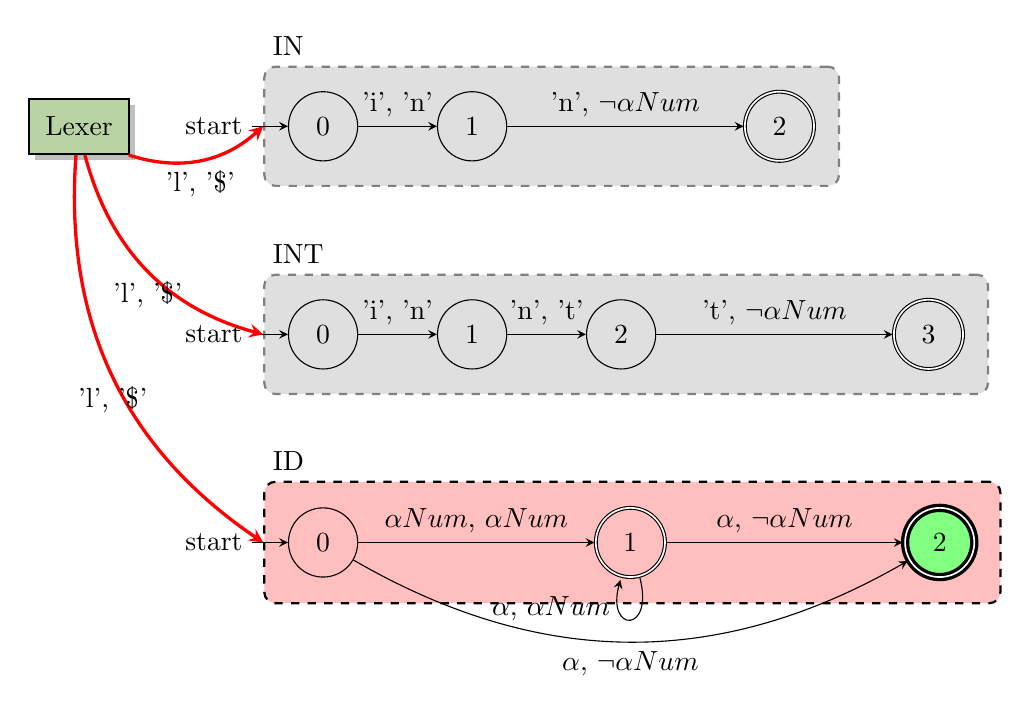
\begin{tikzpicture}[auto,
    ->,
    >=stealth,
    ,
    dead/.style={%
      rectangle, rounded corners=1.5mm, draw=gray, thick, fill=gray!25, drop shadow,align=center,
      text ragged, minimum height=2em, minimum width=2em, inner sep=6pt, outer sep=3pt
    },
    fun/.style = {%
      dashed, draw=black, thick, fill=red!25, rounded corners, rectangle, inner sep=.3cm
    },
    deadfun/.style = {%
      dashed, draw=gray, thick, fill=gray!25, rounded corners, rectangle, inner sep=.3cm
    }
  ]

    \node[bb] (lexer)                           {Lexer};
% IN  
    \node[initial, state]   (10) [right = of lexer, xshift=1cm]          {$0$};
    \node[state]            (11) [right = of 10]             {$1$};
    \node[state, accepting] (12) [right = of 11, xshift=2cm] {$2$};
    
    \path (10) edge node {'i', 'n'} (11)
          (11) edge node {'n', $\neg\alpha Num$} (12)
    ;

% INT
    \node[initial, state]   (20) [below = of 10, yshift = -0.75cm] {$0$};
    \node[state]            (21) [right = of 20] {$1$};
    \node[state]            (22) [right = of 21] {$2$};
    \node[state, accepting] (23) [right = of 22, xshift=2cm] {$3$};
    
    \path (20) edge node {'i', 'n'} (21)
          (21) edge node {'n', 't'} (22)
          (22) edge node {'t', $\neg\alpha Num$} (23)
    ;
    
%ID
    \node[initial, state]   (30) [below = of 20, yshift = -0.75cm] {$0$};
    \node[state, accepting]            (31) [right = of 30, xshift=2cm] {$1$};
    \node[state, accepting, very thick, fill=green!50]            (32) [right = of 31, xshift=2cm] {$2$};
    
    \path (30) edge node {$\alpha Num$, $\alpha Num$} (31)
          (31) edge[loop below] node[near end, left] {$\alpha$, $\alpha Num$} (31)
          (31) edge node[above] {$\alpha$, $\neg\alpha Num$} (32)
          (30) edge[bend right] node[below] {$\alpha$, $\neg\alpha Num$} (32)
	;
	    
    \begin{pgfonlayer}{background}
      \node[deadfun] (in)[fit = (10) (11) (12)] {};
      \node[deadfun] (int)[fit = (20) (21) (22) (23)] {};
      \node[fun] (id)[fit = (30) (31) (32)] {};
      \node[above right] at (in.north west){IN};
      \node[above right] at (int.north west){INT};
      \node[above right] at (id.north west){ID};

    \end{pgfonlayer}
    
	\draw[->, very thick, red, bend right] (lexer) to node[below, black]{'l', '\$'} (in.west);
	\draw[->, very thick, red, bend right] (lexer) to node[below, black]{'l', '\$'} (int.west);
	\draw[->, very thick, red, bend right] (lexer) to node[below, black]{'l', '\$'} (id.west);
	    
  \end{tikzpicture}
}

\end{center}

\end{frame}
% frame end %%%%%%%%%%%%%%%%%%%%%%%%


% frame begin %%%%%%%%%%%%%%%%%%%%%%%%
\begin{frame}{Implementation of Lexical Analysis}
{Manual Implementation of Lexical Analysers}
\myminorheader{Important Points}
\begin{enumerate}
	\item The scanners must be ordered carefully.
	\item Alternative design.
	\begin{itemize}
		\item No separate scanner for keywords
		\item Maintain a table of keywords
		\item On detecting an identifier, check if it's a keyword. If yes, return suitable token. Otherwise, return identifier.
	\end{itemize}
\end{enumerate}
\end{frame}
% frame end %%%%%%%%%%%%%%%%%%%%%%%%


% frame begin %%%%%%%%%%%%%%%%%%%%%%%%
\begin{frame}{Implementation of Lexical Analysis}
{Automatic Generation of Lexical Analysers}
\begin{center}
\resizebox{\textwidth}{!}{%
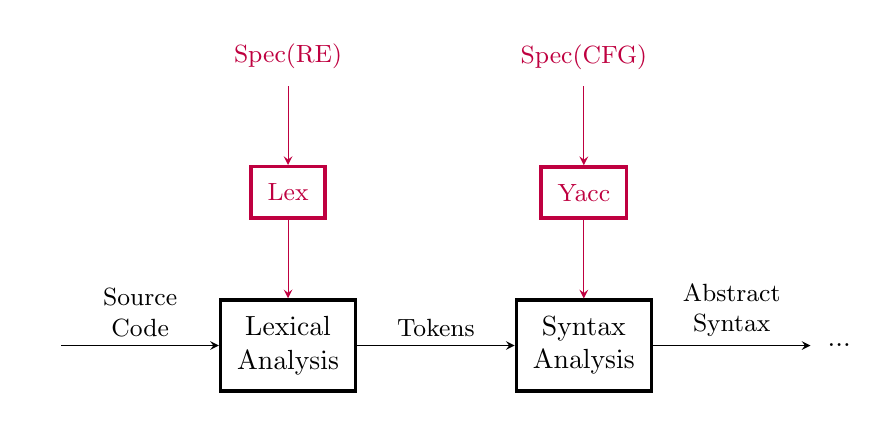
\begin{tikzpicture}[auto,
    ->,
  %  shorten >=2pt,
    >=stealth,
  %  node distance=1cm,
    bb/.style={%
      rectangle, draw=black, very thick, fill=white,
      text ragged, minimum height=2em, inner sep=6pt, align=center
    },
    inv/.style={%
      rectangle, draw=none, fill=white,
      text ragged, minimum height=2em, inner sep=6pt, align=center
    }
]
    \node[inv] (0) []             {};
    \node[bb]  (1) [right = of 0, xshift=1cm] {Lexical \\ Analysis};
    \node[bb]  (2) [right = of 1, xshift=1cm] {Syntax \\ Analysis};
    \node[inv]  (3) [right = of 2, xshift=1cm] {...};

\begin{small}
    \path (0) edge node[align=center] {Source \\ Code}     (1)
          (1) edge node[align=center] {Tokens}             (2)
          (2) edge node[align=center] {Abstract \\ Syntax} (3)
    ;

\pause
    \node[bb, draw=purple, text=purple]  (4) [above = of 1] {Lex};
    \node[inv, text=purple] (6) [above = of 4] {Spec(RE)};

	\path
          (4) edge[purple] node[align=center] {}  (1)
          (6) edge[purple] node[align=center] {}    (4)
	;

\pause
    \node[bb, draw=purple, text=purple]  (5) [above = of 2] {Yacc};
    \node[inv, text=purple] (7) [above = of 5] {Spec(CFG)};

	\path
          (5) edge[purple] node[align=center] {}  (2)
          (7) edge[purple] node[align=center] {}    (5)
	;	
\end{small}
  \end{tikzpicture}
}

\end{center}

\end{frame}
% frame end %%%%%%%%%%%%%%%%%%%%%%%%

\end{document}
